
\section{Entrenamiento}

\begin{frame}
\frametitle{Dataset}
\begin{itemize}
\item<1-> Para entrenar estas redes se necesitan \textbf{decenas de miles de millones} de samples. Generarlo a mano es inviable.
\item<2-> Uso el mismo dataset usado para entrenar Stockfish 16.1 (135GB, 48.4 billion)
\item<3-> Cada sample se ve así:
\begin{center}
\begin{tabular}{|cp{0.0005cm}cp{0.0005cm}c|}
\hline
\textbf{FEN} & , & \textbf{Score} & , & \textbf{Best move} \\
\hline
\end{tabular}
\end{center}
\item<4-> 130 GB → 2 TB → 522 GB
\end{itemize}
\end{frame}

\begin{frame}
\frametitle{Métodos de entrenamiento}
\begin{enumerate}
\item \textbf{Target scores} o \textbf{Score target}: Utiliza las evaluaciones del dataset como target.
\item \textbf{PQR}: Utiliza dos principios \textit{razonables} para armar una función de pérdida.
\end{enumerate}
\end{frame}


\begin{frame}
\frametitle{Score-space a WDL-space}
\begin{itemize}
\item \textbf{Score-space}: los scores en el dataset están entre [-10000, 10000] (\textit{centipawn} o proporcional)
\item \textbf{WDL-space}: otra escala donde 0 es perder, 0.5 es empate y 1 es ganar
\end{itemize}
\pause
Queremos que la red genere valores en \textbf{score-space}, pero para las funciones de pérdida es mejor usar \textbf{WDL-space}.
\end{frame}

\begin{frame}
\frametitle{Score-space a WDL-space}
El modelo WDL dice que el winrate se puede modelar como una función de la evaluación. \pause \\

Los datos muestran que la función sigmoide da una buena aproximación:
\[
\mathcal{W}(f(P)) = \sigma\left(\frac{f(P)-a}{b}\right) = \frac{1}{1 + e^{-\frac{f(P)-a}{b}}}
\]
\end{frame}

\begin{frame}
\frametitle{Score-space a WDL-space}
\begin{figure}[H]
\centering
\makebox[\textwidth]{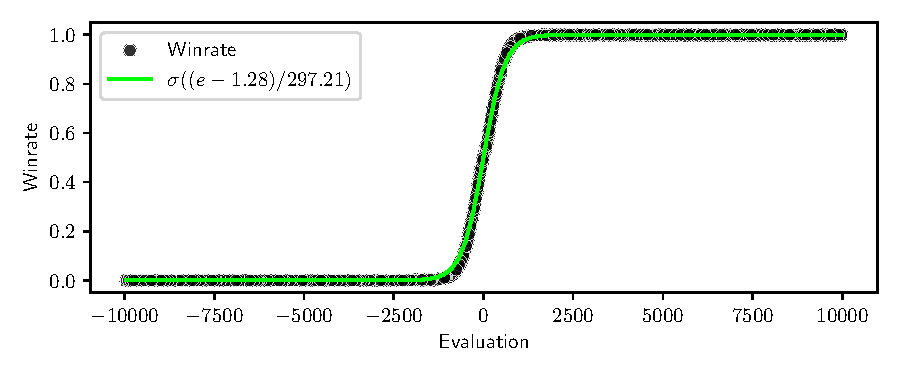
\includegraphics[width=\textwidth]{../assets/sigmoid_fit.pdf}}
\caption{Modelo WDL ajustado a 100 million de evaluaciones en el dataset.}
\end{figure}
\end{frame}

\begin{frame}
\frametitle{Score-space a WDL-space}
¿Para qué WDL? \pause
\begin{itemize}
\item<2-> Las evaluaciones están mas \enquote{cerca} en WDL-space:
\begin{itemize}
\item 7500 vs 8000: 1\% winrate
\item 50 vs 550 : 30\% winrate
\end{itemize}
\item<3-> Se puede interpolar con los resultados (no lo hago)
\begin{itemize}
\item $\lambda \cdot \mathcal{W}(f(P)) + (1 - \lambda) \cdot r$
\end{itemize}
\item<4-> Gradientes más chicos
\end{itemize}

\end{frame}

\begin{frame}
\frametitle{Método 1: Target scores}
Usamos los valores del dataset como target. \pause \\ La función de pérdida es \textbf{Mean Square Error (MSE)} con potencia 2.6.
\[
\mathcal{L}(y,f(x,\bm{W}))= \frac{1}{N} \sum_i^N \left| \mathcal{W}(y_i) - \mathcal{W}(f(x_i,\bm{W})) \right| ^{2.6}
\]
donde\dots

\begin{enumerate}
\itemsep0em
\item $N$ es la cantidad de muestras.
\item $y$ son las evaluaciones objetivo.
\item $f$ es el modelo.
\item $x$ son los inputs (vector del feature sets).
\item $\bm{W}$ son los parámetros del modelo.
\item $\mathcal{W}$ es la función de winrate que mapea de score-space a WDL-space.
\end{enumerate}
\end{frame}


\begin{frame}
\frametitle{Método 2: PQR}
Técnica vista en un blogpost de 2014 por Erik Bernhardsson, que se basa en dos principios: \pause \\
\begin{enumerate}
\item Para dos posiciones en suseción $P \rightarrow Q$ observadas en el dataset, tenemos que \mbox{$f(P)=-f(Q)$}. Esto es porque el juego es de suma cero. \pause
\item Ir desde $P$, no a la posición observada $Q$, sino a una posición \textit{random} $P \rightarrow R$, se debe cumplir $f(R) > f(Q)$ porque un movimiento random es mejor para el siguiente jugador y peor para el que hizo el movimiento.
\end{enumerate}
\pause
Se puede construir una función de pérdida que refleje la igualdad en (1) y la desigualdad en (2).
\end{frame}


\begin{frame}
\frametitle{Método 2: PQR}
% sum of negative log likelihood
La función de pérdida es la suma de la log-verosimilitud negativa de las inecuaciones:
\begin{itemize}
\item ${f(R) > f(Q)}$
\item ${f(P) > - f(Q)}$
\item ${f(P) < -f(Q)}$
\end{itemize}
\end{frame}

\begin{frame}
\frametitle{Método 2: PQR}
\begin{align*}
\mathcal{L}(x^P, x^Q, x^R, \bm{W})=
\frac{1}{N}
\sum_i^N
& -\log\left(\sigma(r_i - q_i)\right) \\
& -\log\left(\sigma(p_i + q_i)\right) \\
& -\log\left(\sigma(-(p_i + q_i))\right)
\end{align*}
\begin{enumerate}
\itemsep0em
\item $x^i$ son los inputs (vector del feature sets) para las posiciones $i \in \{P,Q,R\}$.
\item $\overline{\mathcal{W}}(x) = 2 \mathcal{W}(x) - 1$ es una función que mapea de WDL-space [0, 1] a $[-1, 1]$, así $\overline{\mathcal{W}}(x) = -\overline{\mathcal{W}}(-x)$.
\item $
p_i = \overline{\mathcal{W}}(f(x^P_i, \bm{W})),\text{ }
q_i = \overline{\mathcal{W}}(f(x^Q_i, \bm{W}),\text{ }
r_i = \overline{\mathcal{W}}(f(x^R_i, \bm{W})
$.
\end{enumerate}
\end{frame}


\begin{frame}
\frametitle{Método 2: PQR}
\begin{figure}[H]
\centering
\resizebox{5cm}{5cm}{
    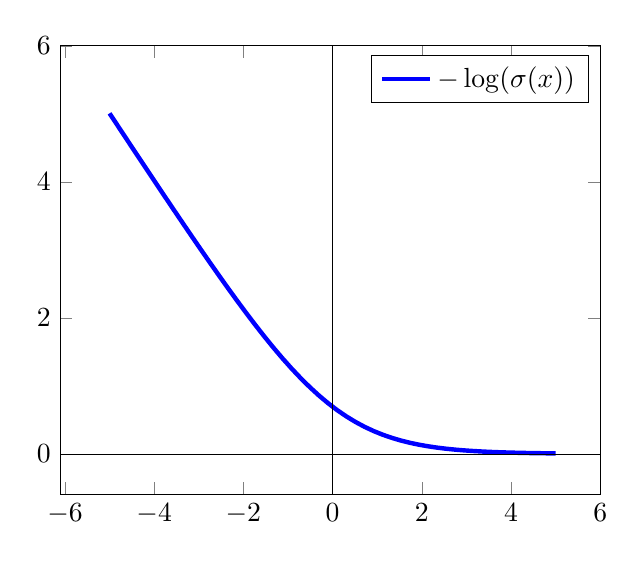
\begin{tikzpicture}
    \begin{axis}[xmax=6,ymax=6, samples=50]
    \addplot[blue, ultra thick] (x,{-ln(1/(1+e^-x))});
    \draw[ultra thin] (axis cs:\pgfkeysvalueof{/pgfplots/xmin},0) -- (axis cs:\pgfkeysvalueof{/pgfplots/xmax},0);
    \draw[ultra thin] (axis cs:0,\pgfkeysvalueof{/pgfplots/ymin}) -- (axis cs:0,\pgfkeysvalueof{/pgfplots/ymax});
    \addlegendentry{$-\log(\sigma(x))$}
    \end{axis}
    \end{tikzpicture}
}
\end{figure}
La función se acerca a 0 cuando $x$ crece y se acerca a $\infty$ cuando $x$ tiende a $-\infty$.
\end{frame}

\begin{frame}
\frametitle{Método 2: PQR}
Veamos cada uno de los términos:
\begin{enumerate}
\itemsep0em
\item $-\log(\sigma(r_i - q_i))$: Este término es chico cuando $r_i > q_i$, y grande cuando $r_i < q_i$.
\item $-\log(\sigma(p_i + q_i))$: Este término es chico cuando $p_i > -q_i$, y grande cuando $p_i < -q_i$.
\item $-\log(\sigma(-(p_i + q_i))$: Este término es chico cuando $p_i < -q_i$, y grande cuando $p_i > -q_i$.
\end{enumerate}

El término (1) sostiene la inecuación $f(R) > f(Q)$, y los términos (2) y (3) la igualdad $f(P) = -f(Q)$.
\end{frame}

\begin{frame}
\frametitle{Setup}
\begin{figure}[H]
\centering
\makebox[\textwidth]{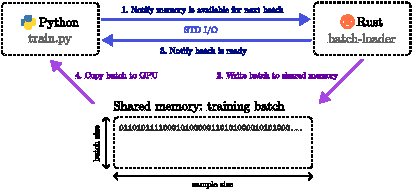
\includegraphics[width=\textwidth]{../assets/training-loop.pdf}}
\caption{Secuencia de pasos para enviar un batch del subproceso \texttt{batch-loader} en Rust a Pytorch.}
\end{figure}
\end{frame}
